%!TEX root = ../cursustekst_fys6.tex

\chapter{Geluid}

\phantom{.}
%vb: stemvork, trommel(vlies)
%
%toonladders, wiskunde en muziek
%
%\section{}
%
%\section{}
%
%\subsection{}

\begin{figure}[h]
\centering
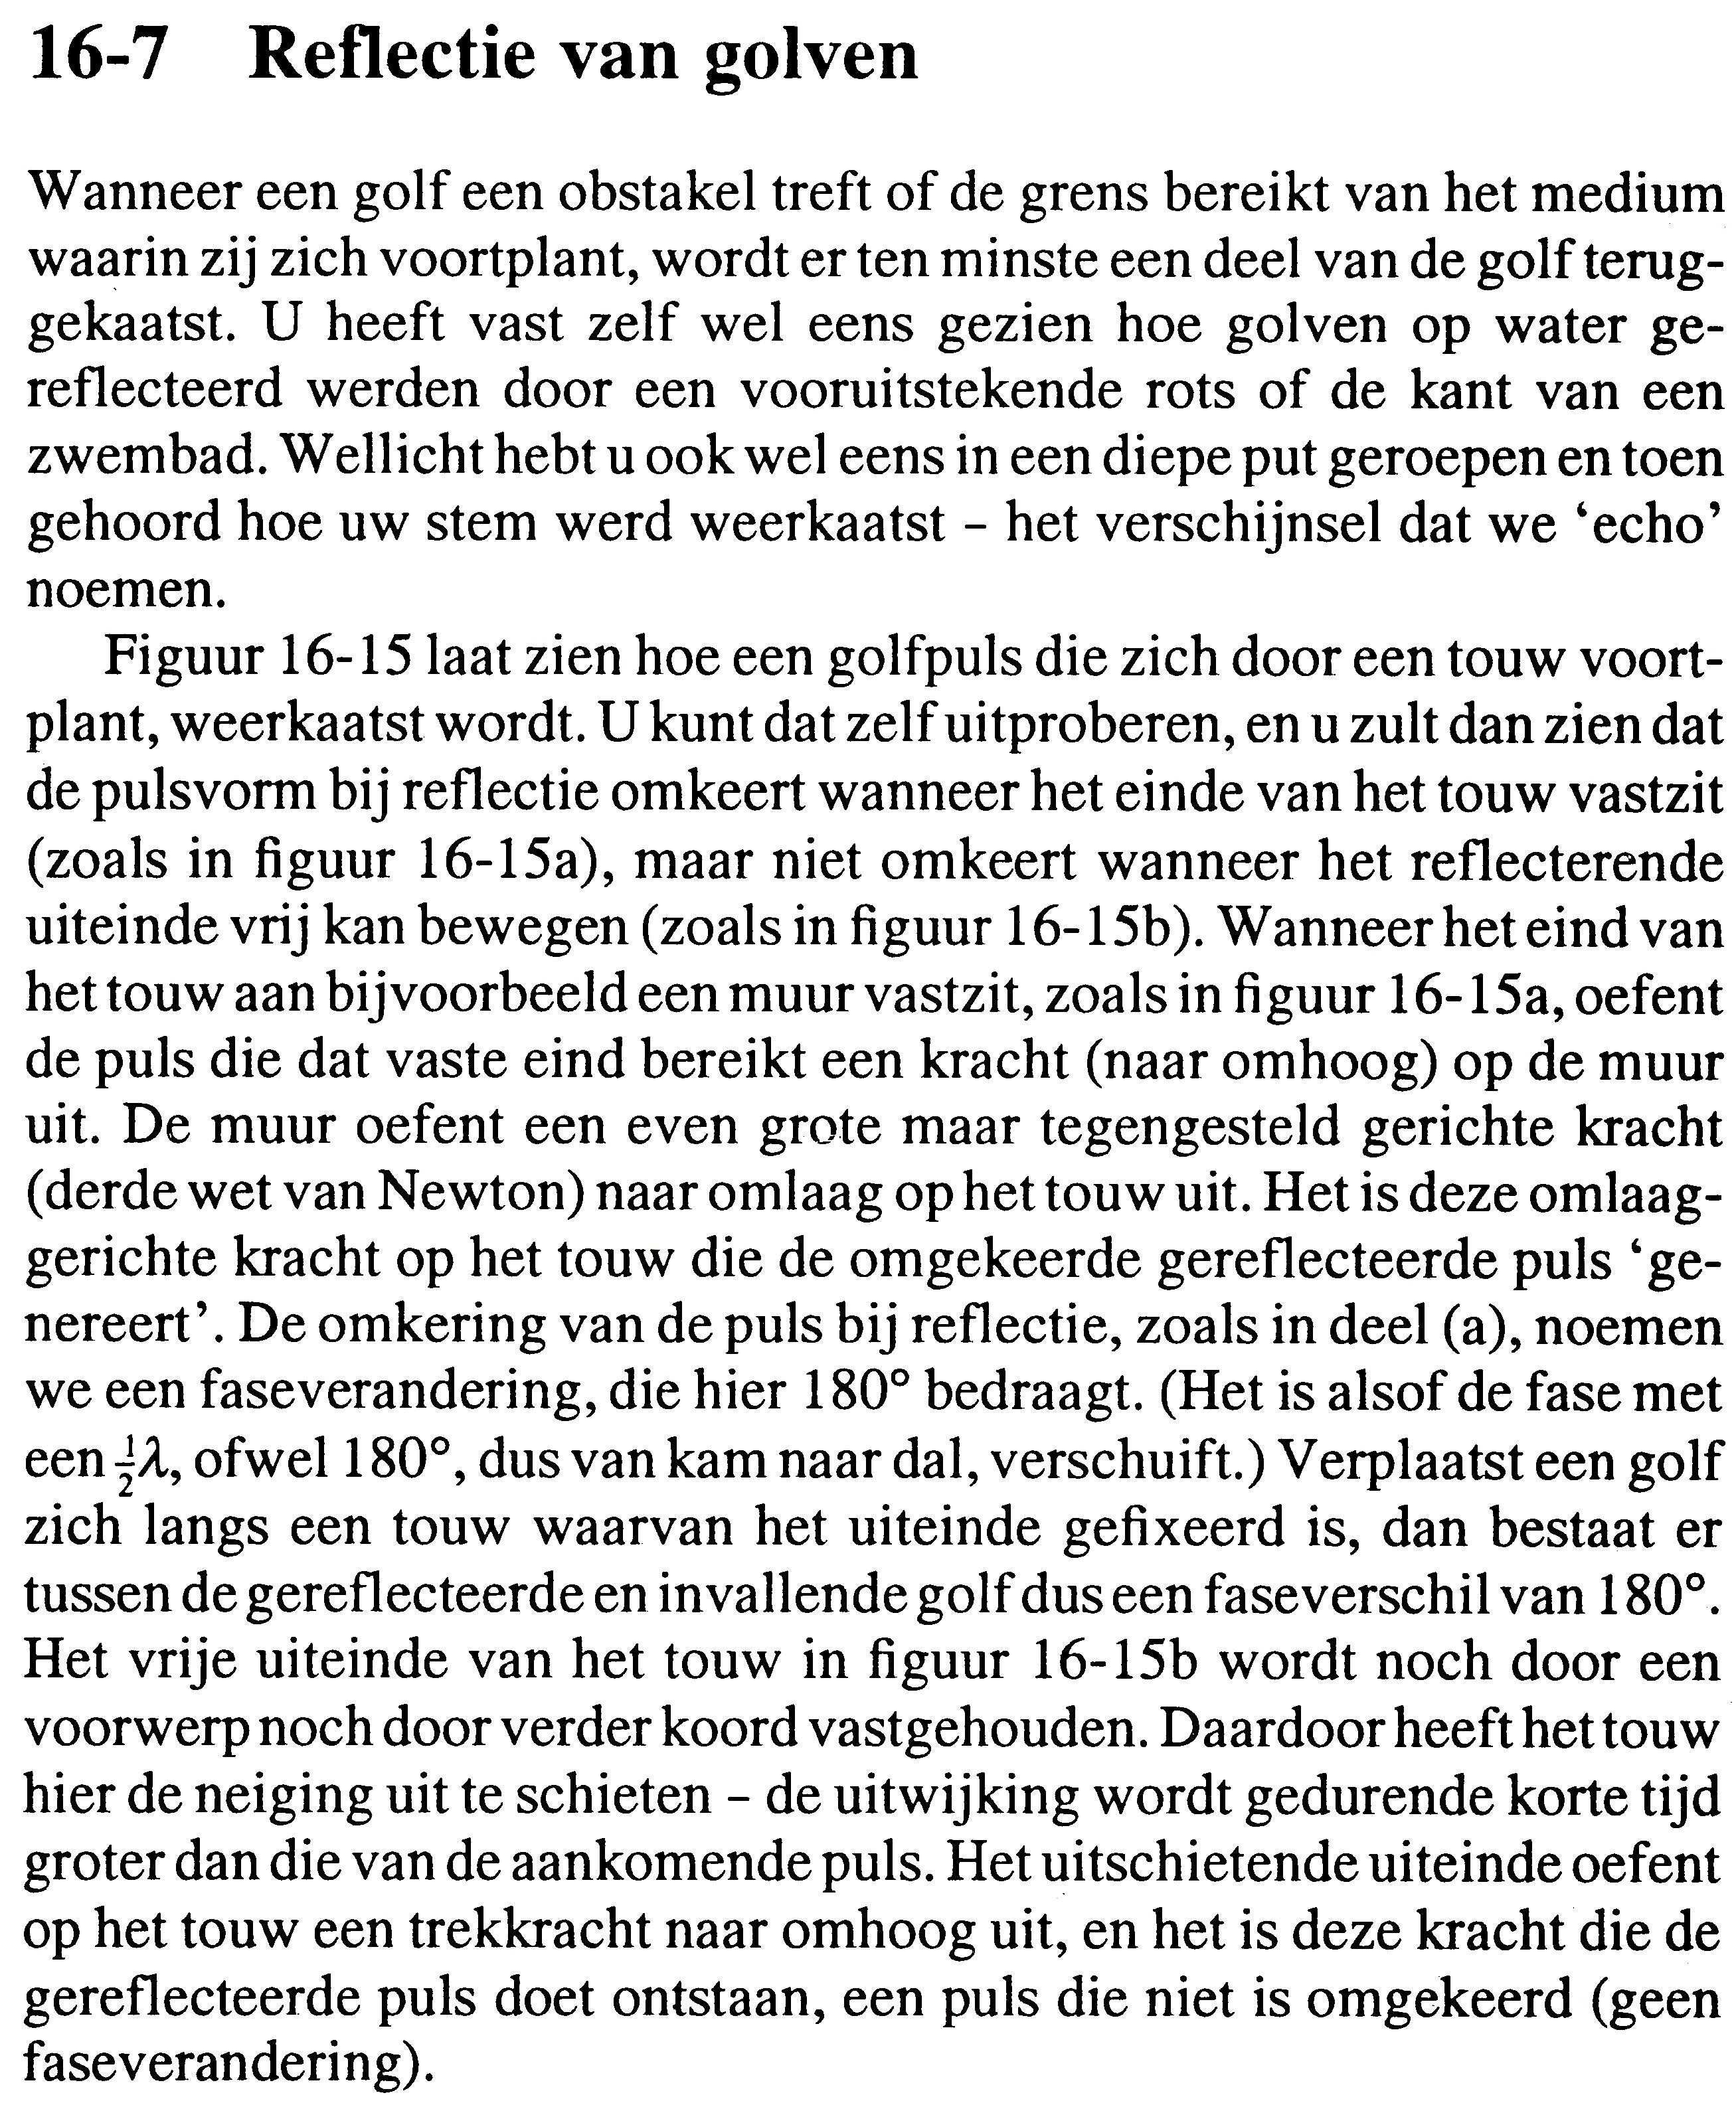
\includegraphics[width=0.8\textwidth]{./geluid_giancoli/scan_0}
\end{figure}

\newpage

\begin{figure}[h]
\centering
\includegraphics[width=1.1\textwidth]{./geluid_giancoli/scan_1}
\end{figure}

\newpage

\begin{figure}[h]
\centering
\includegraphics[width=0.8\textwidth]{./geluid_giancoli/scan_2}
\end{figure}


\begin{figure}[h]
\centering
\includegraphics[width=0.8\textwidth]{./geluid_giancoli/scan_3}
\end{figure}

\begin{figure}[h]
\centering
\includegraphics[width=0.8\textwidth]{./geluid_giancoli/scan_4}
\end{figure}

\begin{figure}[h]
\centering
\includegraphics[width=0.8\textwidth]{./geluid_giancoli/scan_5}
\end{figure}

\begin{figure}[h]
\centering
\includegraphics[width=0.8\textwidth]{./geluid_giancoli/scan_6}
\end{figure}

\begin{figure}[h]
\centering
\includegraphics[width=0.8\textwidth]{./geluid_giancoli/scan_7}
\end{figure}

\begin{figure}[h]
\centering
\includegraphics[width=0.8\textwidth]{./geluid_giancoli/scan_8}
\end{figure}

\begin{figure}[h]
\centering
\includegraphics[width=1.1\textwidth]{./geluid_giancoli/scan_9}
\end{figure}

\begin{figure}[h]
\centering
\includegraphics[width=0.8\textwidth]{./geluid_giancoli/scan_10}
\end{figure}

\begin{figure}[h]
\centering
\includegraphics[width=1.1\textwidth]{./geluid_giancoli/scan_11}
\end{figure}

\begin{figure}[h]
\centering
\includegraphics[width=1.2\textwidth]{./geluid_giancoli/scan_12}
\end{figure}

%\cleardoublepage

\begin{figure}[h]
\centering
\includegraphics[width=0.8\textwidth]{./geluid_giancoli/scan_13}
\end{figure}
\vfill






















